\section*{3.1 范数}
\addcontentsline{toc}{section}{3.1 范数}
\label{sec:3.1}

当我们考虑几何向量（即从原点出发的有向线段）时，向量的长度在直观上就是该有向线段的“端点”到原点的距离。下面，我们将利用 \emph{范数（norm）} 的概念来讨论向量的长度。

\textbf{定义 3.1}（范数）。向量空间 $ V $ 上的 \emph{范数（norm）} 是一个函数：

\begin{equation}
\|\cdot\| : V \to \mathbb{R}
\tag{3.1}\label{eq:3-1}
\end{equation}

\begin{equation}
\boldsymbol{x} \mapsto \|\boldsymbol{x}\|
\tag{3.2}\label{eq:3-2}
\end{equation}

它为每个向量 $ \boldsymbol{x} $ 分配其长度 $ \|\boldsymbol{x}\| \in \mathbb{R} $，使得对于所有 $ \lambda \in \mathbb{R} $ 以及 $ \boldsymbol{x}, \boldsymbol{y} \in V $，满足以下性质：

\begin{itemize}
\item \emph{绝对齐次性（absolutely homogeneous）} ：$ \|\lambda \boldsymbol{x}\| = |\lambda| \|\boldsymbol{x}\| $
\item \emph{三角不等式（triangle inequality）} ：$ \|\boldsymbol{x} + \boldsymbol{y}\| \leqslant \|\boldsymbol{x}\| + \|\boldsymbol{y}\| $
\item \emph{正定性（positive definite）} ：$ \|\boldsymbol{x}\| \geqslant 0 $ 且 $ \|\boldsymbol{x}\| = 0 \iff \boldsymbol{x} = \boldsymbol{0} $
\end{itemize}


\begin{figure}[H]
\centering
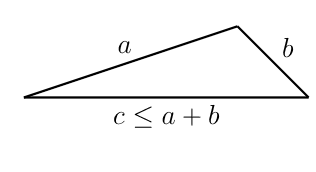
\includegraphics[width=0.92\textwidth,keepaspectratio]{docs/images/Figure3.2.png}
\caption*{\refstepcounter{figcounter}\label{fig:3-2}图~\thefigcounter 三角不等式。}
\end{figure}


从几何意义上讲，三角不等式表明对于任意三角形，任意两边长度之和必须大于或等于第三边的长度；参见图~\ref{fig:3-2} 的示意说明。

定义 3.1 是针对一般向量空间 $ V $（第 2.4 节）给出的，但在本书中，我们将主要考虑有限维向量空间 $ \mathbb{R}^n $。回想一下，对于向量 $ \boldsymbol{x} \in \mathbb{R}^n $，我们使用下标表示该向量的分量，即 $ x_i $ 是向量 $ \boldsymbol{x} $ 的第 $ i $ 个元素。

\begin{notebox}
\textbf{例 3.1（曼哈顿范数）}
\end{notebox}

\begin{notebox}
$ \mathbb{R}^n $ 上的 \emph{曼哈顿范数（Manhattan norm）} 对 $ \boldsymbol{x} \in \mathbb{R}^n $ 定义为：

\begin{equation}
\|\boldsymbol{x}\|_1 := \sum_{i=1}^n |x_i|
\tag{3.3}\label{eq:3-3}
\end{equation}

其中 $ |\cdot| $ 表示绝对值。图~\ref{fig:3-3} 左图显示了 $ \mathbb{R}^2 $ 中所有满足 $ \|\boldsymbol{x}\|_1 = 1 $ 的向量 $ \boldsymbol{x} $。曼哈顿范数也被称为 $ \ell_1 $ 范数（$ \ell_1 $ norm）。
\end{notebox}


\begin{figure}[H]
\centering
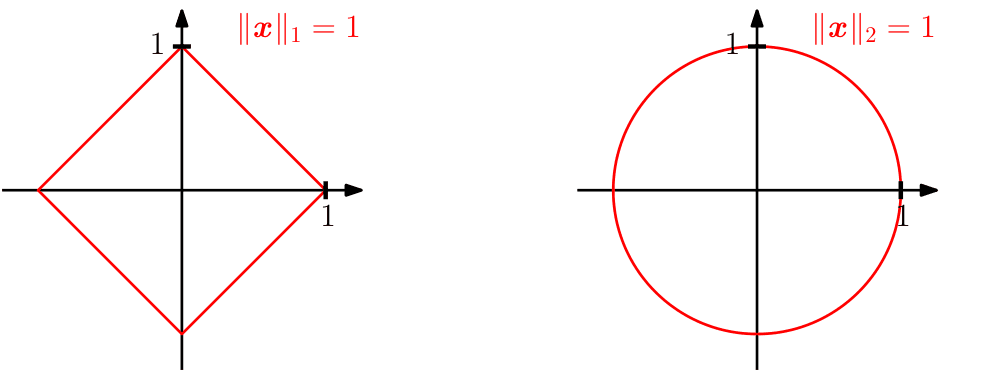
\includegraphics[width=0.92\textwidth,keepaspectratio]{docs/images/Figure3.3.png}
\caption*{\refstepcounter{figcounter}\label{fig:3-3}图~\thefigcounter 对于不同范数，红线表示范数为 1 的向量集合。左图：曼哈顿范数；右图：欧几里得距离。}
\end{figure}


\begin{notebox}
\textbf{例 3.2（欧几里得范数）}
\end{notebox}

\begin{notebox}
$ \boldsymbol{x} \in \mathbb{R}^n $ 的 \emph{欧几里得范数（Euclidean norm）} 定义为：

\begin{equation}
\|\boldsymbol{x}\|_2 := \sqrt{\sum_{i=1}^n x_i^2} = \sqrt{\boldsymbol{x}^\top \boldsymbol{x}}
\tag{3.4}\label{eq:3-4}
\end{equation}

它计算了 $ \boldsymbol{x} $ 到原点的 \emph{欧几里得距离（Euclidean distance）} 。图~\ref{fig:3-3} 右图显示了 $ \mathbb{R}^2 $ 中所有满足 $ \|\boldsymbol{x}\|_2 = 1 $ 的向量 $ \boldsymbol{x} $。欧几里得范数也被称为 $ \ell_2 $ 范数（$ \ell_2 $ norm）。
\end{notebox}

\emph{备注} 。在本书通篇中，若无特殊说明，我们将默认使用欧几里得范数 (3.4)。♦
